\documentclass[12pt]{tlc-article}

% {{{ Begin document

\begin{document}

% -------------------------------------------------------------------------- }}}
% {{{ Abstract and Table of Contents

\tlcTitlePageAndTableOfContents
  {tlc-article}
  {Gary Allan Howard}
  {The \tlcA\ `Getting Started Guide' covers how to install \tlcA\ both globally
   and locally, describes the general use case, how to customize your \tlcA\
   environment, describes the commands \tlcA\ implements, and reveals the
   packages \tlcA\ depends upon.}

% -------------------------------------------------------------------------- }}}
% {{{ Installation

\section{Installation}
This section describes how to install \tlcA\ either globally to make it
available to your \LaTeX\ environment or locally to the document you are
authoring.  And, this section identifies the prerequisites you must meet in
order to clone a repository from GitHub.com and install software on your
computer.

% -------------------------------------------------------------------------- }}}
% {{{ Prerequisites

\subsection{Prerequisites}
The following prerequisites are needed.
\begin{description}[style=nextline]
  \item[Administrative privilege] You will need administrative privileges to
    install \tlcA\ globally because `sudo' is used.

  \item[SSH key] You will need your private key to access \gitHub.  Please refer
    to \url{http://help.github.com/articles/generating-an-ssh-key} for
    instructions on `Generating an SSH key'.

  \item[Enable your SSH key] The following instructions enable your SSH key so
    you to not have to enter the passphrase for each git command.
\end{description}

\begin{lstlisting}[language=bash]
eval \$(ssh-agent -s)
ssh-add ~/.ssh/your-private-key
\end{lstlisting}

% -------------------------------------------------------------------------- }}}
% {{{ Local installation

\subsection{Local installation}
A local installation is done by installing \tlcA\ into
/the/path/to/your/document.  Assuming your document is located at \tlcMyDoc\ the
following shell commands will make \tlcA\ available to your document.

\begin{lstlisting}[language=bash]
cd $HOME
git clone git@GitHub.com:Traap/tlc-article.git
cd tlc-article
mkdir $HOME/mydoc
cp -v tlc-article.cls $HOME/mydoc/.
\end{lstlisting}

% -------------------------------------------------------------------------- }}}
% {{{ Global installation

\clearpage
\subsection{Global installation}
A global installation is done by installing \tlcA\ into your /path/to/your/texmf
directory.  Assuming a TexLive installation exists at \texDist\ the following
shell commands will make \tlcA\ available to your \LaTeX\ environment.

\begin{lstlisting}[language=bash]
cd $HOME
git clone git@GitHub.com:Traap/tlc-article.git
cd tlc-article
sudo mkdir -p $(kpsewhich -var-value TEXMFLOCAL)/tex/latex/tlc-article
sudo cp -v tlc-article.cls $(kpsewhich -var-value TEXMFLOCAL)/tex/latex/tlc-article/.
sudo mktexlsr $(kpsewhich -var-value TEXMFLOCAL)
\end{lstlisting}

\tlcVspace

\todo[inline]{%
  \tlcNote: You may remove your local installation by removing \tlcA.%
}%

% -------------------------------------------------------------------------- }}}
% {{{ General Use Case

\clearpage
\section{General Use Case}
The goal of \tlcA\ is to simplify document layout.  \tlcA\ orchestrates a
logical arrangement for document header, footer, author, abstract, table of
contents, and margins.  The following sections outline the default
implementation for each part \tlcA\ organizes.

\tlcVspace

\tlcNote\ This document was typeset using the instructions provided throughout
this section.

\subsection{Document Layout}
\begin{figure}[h]
  \centering
  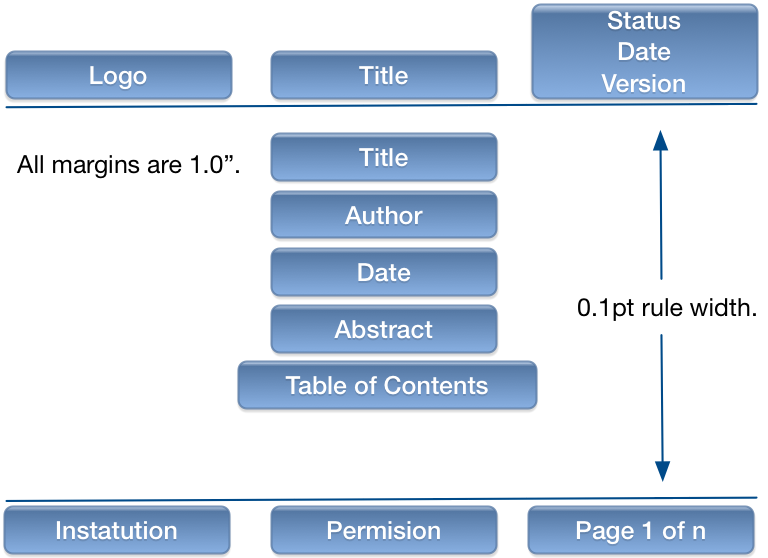
\includegraphics{images/titlepage.png}
  \caption{Document Layout}
  \label{fig:layout}
\end{figure}

% -------------------------------------------------------------------------- }}}
% {{{ Document Class

\subsection{Document Class \tlcA}
\tlcA\ extends the article document class.  \tlcA\ provide options directly to
the article document class.  As an example, the Author can specify the font as
follows:

\begin{lstlisting}[basicstyle=\tiny]
  \documentclass[12pt]{tlc-article}
\end{lstlisting}

% -------------------------------------------------------------------------- }}}
% {{{ Title, Author, and Abstract

\subsection{Title, Author \& Abstract} \label{sec:TAA}
\tlcA\ has a macro \tlcTOC\ that can be used to set the document title, document
author, document abstract, and establish the Table of Contents.  The sample
below reveals how to use \tlcTOC.

\begin{lstlisting}[basicstyle=\tiny]
  \tlcTitlePageAndTableOfContents
     {Document Title}
     {Document Article}
     {Document Abstract}
\end{lstlisting}

% -------------------------------------------------------------------------- }}}
% {{{ Table of Contents

\subsection{Table of Contents}
The Table of Contents immediately follows the document abstract on page 1, uses
dark blue for content, dots separate table of contents sections and page number,
and uses roman numerals.

% -------------------------------------------------------------------------- }}}
% {{{ Header and Footer

\subsection{Header \& Footer}
fancyhdr is used to render the header and footer.  The Author can override the
\tlcA\ by providing an implementation in \tlcHF\, or augment \tlcA\
application by providing \tlcVE. The sections below show the placement \tlcA\
uses when writing objects, and where the objects are defined.

\tlcVspace

\todo[inline]{%
  \tlcNote: \tlcA\ ignores \tlcVE\ when \tlcHF\ is defined.
}%

% -------------------------------------------------------------------------- }}}
% {{{ Header

\subsubsection*{Header}
\begin{description}
  \item[lhead] When \tlcLG\ is found, logo.
  \item[chead] Document Title
  \item[rhead] When \tlcVE\ is present, status, date, and version columns.
\end{description}

% -------------------------------------------------------------------------- }}}
% {{{ Footer

\subsubsection*{Footer}
\begin{description}
  \item[lfoot] When \tlcVE\ is present, institution column.
  \item[cfoot] When \tlcVE\ is present, permission column.
  \item[rfoot] Page 1 of N.
\end{description}

% -------------------------------------------------------------------------- }}}
% {{{ Rule width

\subsubsection*{Rule width}
A 0.1pt rule width is placed below the document header and above the document
footer.

% -------------------------------------------------------------------------- }}}
% {{{ Customization

\clearpage
\section{Customization}
This section describes how \tlcA\ can be customized by using the file-hooks
\tlcA\ check for.  \tlcA\ default implementation will be used when the
file-hooks are not found.

\tlcVspace

\todo[inline]{%
  \tlcNote: \tlcA\ consumes \tlcAL\ \& \tlcHF\ during the preamble compilation
  phase.
}%

% -------------------------------------------------------------------------- }}}
% {{{ data/additional-layout.tex

\subsection{\tlcAL}
\tlcA\ will use whatever \LaTeX\ definitions are found in \tlcAL\ when it
exists.  The file-check is shown
below:

\begin{lstlisting}[basicstyle=\tiny]
  \IfFileExists{data/additional-layout.tex}
    {% This use case demonstrates tlc-article being extended.  All definitions are
% process during preamble phase.  In other words, before your \begin{document}
% statement.

% ------------------------------------------------------------------------------
% \makeatletter is used so we can reference commands and definitions defined by
% tlc-article, which are all prefaced with tlc@.
\makeatletter

% ------------------------------------------------------------------------------
% tlc-article.tex (Getting Starting) definitions.

\def\tlcProduct{tlc-article}%

\def\tlcA{\tlcDarkblue{\tlcProduct}}%

\def\tlcAL{\tlcDarkblue{\tlc@additionalLayout}}%
\def\tlcBL{\tlcDarkblue{tlcBeginLandscape}}%
\def\tlcDB{\tlcDarkblue{tlcDarkblue}}%
\def\tlcEL{\tlcDarkblue{tlcEndLandScape}}%
\def\tlcHF{\tlcDarkblue{\tlc@headerFooter}}%
\def\tlcLG{\tlcDarkblue{\tlc@logoFile}}%
\def\tlcNCT{newcolumn type: \tlcDarkblue{L, C} \& \tlcDarkblue{R}}%
\def\tlcTOC{\tlcDarkblue{tlcTitlePageAndTableOfContents}}%
\def\tlcVE{\tlcDarkblue{\tlc@versionFile}}%

\def\tlcVC{\tlcDarkblue{tlc@version}}%
\def\tlcDC{\tlcDarkblue{tlc@date}}%
\def\tlcSC{\tlcDarkblue{tlc@status}}%
\def\tlcIC{\tlcDarkblue{tlc@instatution}}%
\def\tlcPC{\tlcDarkblue{tlc@permission}}%

\def\kpse{\$(kpsewhich -var-value TEXMFLOCAL)}%
\def\texDist{\kpse}%
\def\tlcDist{/tex/latex/\tlcProduct}%
\def\tlcGlobalDist{\texDist\tlcDist}%

\def\tlcHome{\$HOME}%
\def\tlcMyDoc{\tlcHome/mydoc}%

\def\gitHub{GitHub.com}%
\def\gitHubUrl{http://\gitHub}%

\def\tlcRepo{git@\gitHub:Traap/\tlcProduct.git}%

\def\tlcPkgFile{data/required-packages.csv}%
\def\tlcNote{\tlcDarkblue{Note}}%

% ------------------------------------------------------------------------------%
% Define the column names used by csvreader when reading \packageFile.
\csvnames{tlcPkgNames}{
   1=\name
  ,2=\description
}

% Define the table style used to report the required package names and
% descriptions.
\csvstyle{tlcPkgStyle}{
  longtable=|L{3cm}|L{12cm}|
  ,table head=\hline Name & Description\\\hline\hline\endhead
  ,late after line=\\\hline
  ,tlcPkgNames
}

% ------------------------------------------------------------------------------%
}
    {}
\end{lstlisting}

% -------------------------------------------------------------------------- }}}
% {{{ data/header-footer.tex

\subsection{\tlcHF}
In the absence of \tlcHF, \tlcA\ has a builtin header and footer strategy that
is base on \textit{fancyhdr}, \textit{titling}, and \textit{lastpage} \LaTeX\
packages. The default implementation is show below:

\begin{lstlisting}[basicstyle=\tiny]

\IfFileExists{\tlc@headerFooter}%
{% use the customer header and footer defined by \tlc@headerfooter
  \input{\tlc@headerFooter}%
}%
{% Else : user default header and footer
  \useDefaultHeaderFooter%
}%

\newcommand{\useDefaultHeaderFooter}{%
  \useLogoFile%              Typeset Logo in the left side of the header.
  \chead{\large{\thetitle}}% Typeset title in center of the header.
  \useVersionFile%           Typeset version info in right side of the header.
  \useRuler%                 Typeset header and footer with a ruler.
}%

\newcommand{\useLogoFile}{%
  \IfFileExists{\tlc@logoFile}%
  {%
    \lhead{\includegraphics[width=3cm,height=1cm]{\tlc@logoFile}}%
  }%
  {%
   % Else: no operation because tlc@logoFile does not exist.
  }%
}%

\newcommand{\useVersionFile}{%
  \IfFileExists{\tlc@versionFile}%
  {%
   % document status, document date and document version.
    \rhead{\tiny \tlc@status \\ \tlc@date \\ \tlc@version}%
   %
   % document owner.  This maybe a person or company name.
    \lfoot{\tiny \tlc@institution}%
   %
   % document license. This maybe a license or word like confidential.
    \cfoot{\tiny \tlc@permission}%
  }%
  {%
   % Else: no operation because tlc@versionFile does not exist.
  }%
}%

\newcommand{\useRuler}{%
  \renewcommand{\headrulewidth}{0.1pt}%
  \setlength\headheight{34.0pt}%
  \rfoot%
    {\tiny%
      {Page \thepage~of~\pageref{LastPage}}%
    }%
  \renewcommand{\footrulewidth}{0.1pt}%
}%

\end{lstlisting}

The default implementation can be overridden by defining \tlcHF.

\tlcVspace

\todo[inline]{%
  \tlcNote: When \tlcHF\ exists and is empty, your document will be typeset with
  the defaults from document-class \tlcDarkblue{article}.
}%

% -------------------------------------------------------------------------- }}}
% {{{ data/version.csv

\clearpage
\subsection{\tlcVE} \label{sec:version}
\tlcA\ will populate the builtin header and footer with information extracted
from \tlcVE\ when it is present.  \tlcVE\ is a comma-separated-variable file
that uses the pipe character as the field delimiter.  \tlcVE\ uses the following
column names:

\begin{description}[style=nextline]
  \item[version] The version value is typeset in the rhead area.  This field is
    used to convey the version the document was at the date it reached its
    current state.

  \item[date] The date value is typeset in the rhead area.  This field is used
    to communicate when the document transitioned into its current state.

  \item[status] The status value is typeset in the rhead area.  This field is
    used to convey the document state such as Approved, Draft, Effective, or
    Obsolete.

  \item[instatution] The institution value is typeset in the lfoot area.  This
    field is used to tell the reader the author name or company name.

  \item[permission]  The permission value is typeset in the cfoot area.  This
    field is used to identify confidentiality or a particular license.

\end{description}

The exaction methods are shown below.
\begin{lstlisting}[basicstyle=\tiny]
  % Extract document status, document date and document version from
  % \tlc@versionFile.
  % Argument:
  %   1 - the column name to extract from the data file.
  \newcommand{\tlcVersionPart}[1]{
    \csvreader[separator=pipe]
    {\tlc@versionFile}{
      1=\version,
      2=\date,
      3=\status,
      4=\instatution,
      5=\permission
    }{#1}
  }%

  % Define extractions macros when \tlc@versionFile exists.
  \IfFileExists{\tlc@versionFile}
  {
    \def\tlc@version{\tlcVersionPart{\version}}
    \def\tlc@date{\tlcVersionPart{\date}}
    \def\tlc@status{\tlcVersionPart{\status}}
    \def\tlc@instatution{\tlcVersionPart{\version}}
    \def\tlc@permission{\tlcVersionPart{\version}}
  }
  {% Else: no operation because tlc@versionFile does not exist.
  }
\end{lstlisting}

% -------------------------------------------------------------------------- }}}
% {{{ data/logo.png

\subsection{\tlcLG}
\tlcA\ will typeset the lhead area with \tlcLG\ when it is present. Make sure
your logo's height is not larger than 34pt to avoid `Package Fancyhdr Warning:
\\headheight is to small' warning.

% -------------------------------------------------------------------------- }}}
% {{{ Definitions and Commands

\clearpage
\section{Definitions \& Commands}

% -------------------------------------------------------------------------- }}}
% {{{ tlcBeginLandscape

\subsection{\tlcBL}
Page layout is rotated 90\textdegree\ clockwise resulting in a landscape page
orientation.  Landscape orientation remains active until \tlcEL.

% -------------------------------------------------------------------------- }}}
% {{{ tlcEndLandscape

\subsection{\tlcEL}
Page layout is returned to portrait orientation when \tlcEL\ is reached.

% -------------------------------------------------------------------------- }}}
% {{{ tlcDarkblue

\subsection{\tlcDB}
\tlcDB\ is used throughout this document to render text using rbg\{0,0,0.5\}.
\tlcDB\ is safe to use within your document.

% -------------------------------------------------------------------------- }}}
% {{{ tlcTitlePageAndTableOfContents

\subsection{\tlcTOC}
\tlcTOC\ creates the document layout shown in Figure \ref{fig:layout}.  Section
\ref{sec:TAA} shows an example implementation.

% -------------------------------------------------------------------------- }}}
% {{{ newcolumntype type: L, C and R

\subsection{\tlcNCT}
New \tlcNCT\ are Left, Center, and Right, respectively are
designed to use with longtable.  Data is wrapped within a table cell.   The
parameter defines the column width.  As an example, L{2cm} yields a Left
aligned, ragged right, wrapped text within a 2cm wide cell.

\begin{lstlisting}[basicstyle=\tiny]
\newcolumntype{L}[1]{>{\raggedright\let\newline\\\arraybackslash}p{#1}}
\newcolumntype{C}[1]{>{\centering\let\newline\\\arraybackslash}p{#1}}
\newcolumntype{R}[1]{>{\raggedleft\let\newline\\\arraybackslash}p{#1}}
\end{lstlisting}

% -------------------------------------------------------------------------- }}}
% {{{ data/additional-layout.tex

\subsection{\tlcAL}
\tlcAL\ is an architectural hook the Author should use when it becomes necessary
to use packages not provided by \tlcA\, and to design commands that are specific
to your document.

% -------------------------------------------------------------------------- }}}
% {{{ data/.tex

\subsection{\tlcHF}
\tlcHF\ is an architectural hook the Author should use to completely override
the document layout \tlcA\ implements.

% -------------------------------------------------------------------------- }}}
% {{{ data/version.csv

\clearpage
\subsection{\tlcVE}
\tlcVE\ is by used \tlcA\ to populate the document header \& footer.  Refer to
section \ref{sec:version} for \tlcVE\ definitions. \tlcVE\ is not
used by \tlcA\ when \tlcHF\ is define.  However, you might want to use the
version hook by defining \tlcVE\ and using the commands below to extract data
from \tlcVE\ in your \tlcHF.
\begin{enumerate}
  \item \tlcVC\
  \item \tlcDC\
  \item \tlcSC\
  \item \tlcIC\
  \item \tlcPC\
\end{enumerate}

% -------------------------------------------------------------------------- }}}
% {{{ data/logo.png

\subsection{\tlcLG}
\tlcA\ places \tlcLG\ in your header when defined.

% -------------------------------------------------------------------------- }}}
% {{{ Required Packages

\clearpage
\section{Required Packages}
This section documents the dependencies of the required package tlc-article has.
Package names are listed in alphabetical order. A complete description of each
package is found at \url{http://www.ctan.org/}. At this writing, you can type in
the package name and press the search button to learn more about each package.

% Render pckFile using pckStyle as a longtable.
\csvreader[tlcPkgStyle, separator=pipe]{\tlcPkgFile}{}{\name & \description}

% -------------------------------------------------------------------------- }}}

\end{document}
